% Provenance (never printed): old seconde/premiere S material on the
% atmosphere (storms, cyclones, the energy of the water cycle) and the
% natural-hazard themes of SVT; see sources/book2/PROVENANCE.md. Tracks,
% genesis statistics and the pressure--wind relation are computed in
% figdata/grade-10/cyclones.py from IBTrACS v04r01; the surge, thunder and
% energy numbers in the same script.
\chapter{Orages et cyclones tropicaux}\label{ch:g10:storms-and-cyclones}

Un chaud après-midi d'été s'achève par un \omterm{def:g10:storms-and-cyclones:thunderstorm}{orage}. Le ciel s'assombrit, une
rafale de vent froid balaie la rue, un \omterm{def:g10:storms-and-cyclones:lightning}{éclair} illumine les nuages --- et
l'on se met à compter~: un, deux, trois, \ldots{} neuf secondes plus tard,
le tonnerre gronde. L'\omterm{def:g10:storms-and-cyclones:thunderstorm}{orage} est à environ trois kilomètres. Dans une heure,
il sera passé, et l'air sera frais et pur. Au-dessus des océans tropicaux
chauds, les mêmes ingrédients --- de l'air chaud et humide qui monte et se
condense --- peuvent s'organiser en tempêtes d'une tout autre taille~: les
\omterm{def:g10:storms-and-cyclones:tropical-cyclone}{cyclones tropicaux}, larges de centaines de kilomètres, qui durent des jours
et apportent des vents capables de coucher des forêts et une montée de la
mer qui inonde des côtes entières. Ce chapitre étudie les \omterm{def:g10:storms-and-cyclones:thunderstorm}{orages}, les
\omterm{def:g10:storms-and-cyclones:tornado}{tornades} et les \omterm{def:g10:storms-and-cyclones:tropical-cyclone}{cyclones tropicaux}, et l'origine de leur énergie.

\begin{safety}
Si l'on entend le tonnerre, la foudre peut nous atteindre. Il faut entrer
dans un bâtiment ou dans une voiture fermée et y rester bien après le
dernier coup de tonnerre. Ne jamais s'abriter sous un arbre isolé, et
s'éloigner des sommets, des champs dégagés et de l'eau.
\end{safety}

\begin{recall}
Les masses d'air, les fronts, les dépressions (zones de basse pression) et
les anticyclones sont tracés sur les cartes météorologiques avec des
isobares, lignes d'égale pression (livre~1, année~8). Un risque naturel est
un événement naturel qui peut nuire aux personnes et à ce qu'elles
construisent (livre~1, année~5). Le son se propage dans l'air à environ
\qty{340}{m/s}, la lumière presque instantanément (les livres de physique).
L'air chaud et humide qui monte se refroidit, se condense en nuage à son
\omterm{def:g10:why-clouds-form:condensation-level}{niveau de condensation} et libère de la \omterm{def:g10:earth-energy-budget:latent-heat}{chaleur latente}~; l'air saturé est
souvent instable (\cref{ch:g10:why-clouds-form}).
\end{recall}

\section{Les orages}

\begin{definition}[Orage]\label{def:g10:storms-and-cyclones:thunderstorm}
Un \emph{orage}\index{orage} est une perturbation produite par un nuage
cumulonimbus, avec \omterm{def:g10:storms-and-cyclones:lightning}{éclairs} et tonnerre, accompagnée en général de fortes
averses et de rafales de vent, parfois de grêle.
\end{definition}

Un \omterm{def:g10:storms-and-cyclones:thunderstorm}{orage} naît d'un \omterm{def:g10:why-clouds-form:stability}{air instable} et humide. Dans un premier stade, un cumulus
grandit vers le haut, alimenté par un fort courant ascendant~; la
condensation libère de la \omterm{def:g10:earth-energy-budget:latent-heat}{chaleur latente} et maintient l'air qui monte plus
chaud que son environnement. Au stade de maturité, le nuage atteint l'\omterm{def:g10:why-clouds-form:stability}{air
stable} situé très haut et s'étale en enclume~; gouttes et grêlons
deviennent assez gros pour tomber, et la pluie qui tombe entraîne de l'air
froid avec elle~: un courant descendant qui s'étale au sol en un front de
rafales froid. Au dernier stade, le courant descendant envahit tout le
nuage, coupe l'apport d'air chaud et humide, et l'\omterm{def:g10:storms-and-cyclones:thunderstorm}{orage} s'épuise en pluie.

\begin{omfigure}
\begin{tikzpicture}[font=\footnotesize, >={Stealth[length=2mm]}]
  \foreach \dx/\title in {0/{1. croissance}, 4.6/{2. maturité}, 9.2/{3. dissipation}}
    \node[anchor=north] at (\dx+1.6,-0.15) {\title};
  \draw[thick, black!60] (-0.3,0) -- (12.9,0);
  % stage 1: a tall cumulus
  \pic[scale=1.4, transform shape] at (1.6,1.2) {puffycloud};
  \pic[scale=1.1, transform shape] at (1.6,2.0) {puffycloud};
  \foreach \x in {1.2,1.6,2.0} \draw[->, thick, omThm!80!black] (\x,0.2) -- (\x,2.6);
  % stage 2: cumulonimbus with anvil
  \fill[black!8, draw=black!50] (5.0,1.0) -- (4.9,4.0) -- (4.2,4.4) -- (8.0,4.6) -- (7.4,4.0) -- (7.2,1.0) -- cycle;
  \draw[->, thick, omThm!80!black] (5.5,0.2) -- (5.5,4.2);
  \draw[->, thick, omThm!80!black] (5.9,0.2) -- (5.9,4.2);
  \draw[->, thick, omDef!80!black] (6.7,3.4) -- (6.7,0.3) -- (7.6,0.3);
  \foreach \x in {6.4,6.85,7.05} \draw[omDef!50] (\x,0.95) -- (\x-0.1,0.1);
  \node[anchor=west, align=left] at (8.0,4.6) {enclume};
  \node[anchor=west, align=left, omDef!80!black] at (7.65,0.45) {front de rafales};
  % stage 3: dissipating
  \fill[black!8, draw=black!50] (9.7,1.2) -- (9.6,3.6) -- (9.0,4.0) -- (12.6,4.1) -- (12.0,3.6) -- (11.8,1.2) -- cycle;
  \foreach \x in {10.3,10.9,11.5} \draw[->, thick, omDef!80!black] (\x,3.2) -- (\x,0.3);
  \foreach \x in {10.6,11.2} \draw[omDef!50] (\x,1.15) -- (\x-0.1,0.1);
  % legend
  \draw[->, thick, omThm!80!black] (0,5.0) -- (0,5.5); \node[anchor=west] at (0.1,5.25) {ascendance chaude};
  \draw[->, thick, omDef!80!black] (3.2,5.5) -- (3.2,5.0); \node[anchor=west] at (3.3,5.25) {descendance froide};
\end{tikzpicture}

{\small Les trois stades d'un \omterm{def:g10:storms-and-cyclones:thunderstorm}{orage} (schéma, sans échelle)~: un cumulus en
croissance, alimenté par des courants ascendants~; le cumulonimbus mûr, avec
son enclume, son courant ascendant et un courant descendant entraîné par la
pluie~; l'\omterm{def:g10:storms-and-cyclones:thunderstorm}{orage} qui se dissipe, entièrement descendant.}
\end{omfigure}

Dans le nuage, les collisions entre particules de glace emportées vers le
haut et vers le bas par l'air séparent des charges électriques~: le nuage
se charge, en général négativement à sa base et positivement à son sommet,
et le sol sous lui acquiert lui aussi une charge.

\begin{definition}[Éclair]\label{def:g10:storms-and-cyclones:lightning}
Un \emph{éclair}\index{eclair@éclair} est une gigantesque étincelle
électrique qui décharge des régions chargées d'un \omterm{def:g10:storms-and-cyclones:thunderstorm}{orage}, à l'intérieur du
nuage, entre nuages, ou entre le nuage et le sol. Il chauffe un étroit canal
d'air si brusquement que l'air se dilate avec un choc~: le bruit de cette
dilatation est le \emph{tonnerre}.
\end{definition}

\begin{omfigure}
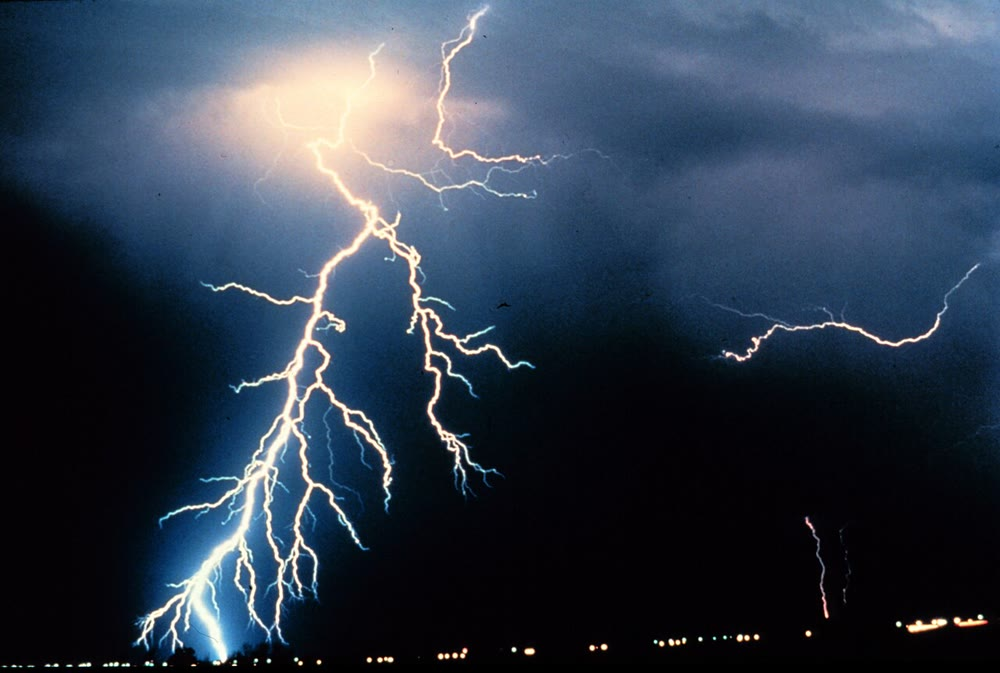
\includegraphics[width=0.62\linewidth]{images/book2/g10-noaa-lightning.jpg}

{\small Des \omterm{def:g10:storms-and-cyclones:lightning}{éclairs}, entre nuages et du nuage au sol, pendant un \omterm{def:g10:storms-and-cyclones:thunderstorm}{orage}
nocturne. Photographie~: C.~Clark, NOAA National Severe Storms Laboratory
(domaine public).}
\end{omfigure}

Les satellites qui comptent les \omterm{def:g10:storms-and-cyclones:lightning}{éclairs} de lumière sur toute la planète en
trouvent environ 1.4~milliard par an, soit 44 chaque seconde.
% ledger: christian:flash-rate

\begin{method}[Distance d'un orage, de l'éclair au tonnerre]\label{met:g10:storms-and-cyclones:distance}
\begin{enumerate}
  \item La lumière de l'\omterm{def:g10:storms-and-cyclones:lightning}{éclair} arrive pratiquement aussitôt~; le tonnerre
        se propage à la vitesse du son, environ \qty{343}{m/s} à
        \qty{20}{\degreeCelsius}.
  \item Compter les secondes $t$ entre l'\omterm{def:g10:storms-and-cyclones:lightning}{éclair} et le tonnerre.
  \item La distance vaut $343\,t$ mètres~: environ \qty{1}{km} toutes les
        trois secondes.
\end{enumerate}
\end{method}
% ledger: const:R, earth:Mmol (speed of sound computed in figdata/grade-10/cyclones.py)

\section{Les tornades}

\begin{definition}[Tornade]\label{def:g10:storms-and-cyclones:tornado}
Une \emph{tornade}\index{tornade} est une colonne d'air en rotation
violente, en contact avec le sol, suspendue à la base d'un cumulonimbus.
\end{definition}

Les \omterm{def:g10:storms-and-cyclones:tornado}{tornades} les plus fortes viennent des \emph{supercellules}, des \omterm{def:g10:storms-and-cyclones:thunderstorm}{orages}
dont le courant ascendant tourne tout entier. Une \omterm{def:g10:storms-and-cyclones:tornado}{tornade} est petite et
brève~: typiquement quelques centaines de mètres de large, elle dure
quelques minutes, sur une trajectoire moyenne d'environ \qty{5.6}{km}. Mais
ses vents sont les plus forts de la surface terrestre~: un radar mobile a
mesuré environ \qty{135}{m/s} (quelque \qty{480}{km/h}) au-dessus du sol
dans une \omterm{def:g10:storms-and-cyclones:tornado}{tornade} de l'Oklahoma en mai 1999. Les États-Unis comptent plus de
\omterm{def:g10:storms-and-cyclones:tornado}{tornades} que tout autre pays, environ 1200 par an~; elles sont fréquentes
aussi dans les prairies canadiennes, au Bangladesh, dans le nord de
l'Argentine et le sud du Brésil, et en Grande-Bretagne.
% ledger: spc:tornado

\begin{omfigure}
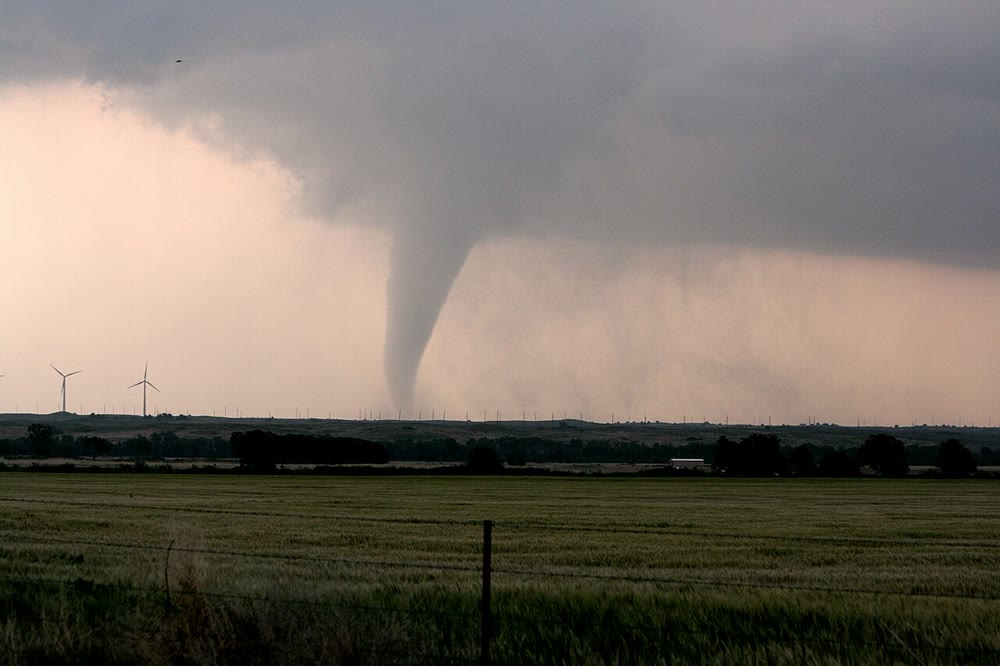
\includegraphics[width=0.62\linewidth]{images/book2/g10-noaa-tornado-kansas.jpg}

{\small Une \omterm{def:g10:storms-and-cyclones:tornado}{tornade} au-dessus des plaines du Kansas, mai 2008~: l'entonnoir
pend de la base du nuage d'\omterm{def:g10:storms-and-cyclones:thunderstorm}{orage}. Photographie~: Sean Waugh, NOAA National
Severe Storms Laboratory (domaine public).}
\end{omfigure}

\section{Les cyclones tropicaux}

\begin{definition}[Cyclone tropical~; œil~; mur de l'œil]\label{def:g10:storms-and-cyclones:tropical-cyclone}
Un \emph{cyclone tropical}\index{cyclone tropical} est une tempête, large
de centaines de kilomètres, qui se forme au-dessus d'une mer tropicale
chaude autour d'un centre de basse pression, avec des vents qui spiralent
vers le centre et des bandes orageuses. Quand ses vents soutenus atteignent
\num{64}~nœuds, environ \qty{119}{km/h}, on l'appelle ouragan dans
l'Atlantique et le Pacifique Est, typhon dans le Pacifique Ouest, et
simplement cyclone dans l'océan Indien et le Pacifique Sud. Son centre
calme, presque sans nuages, est l'\emph{œil}\index{oeil@œil}~; l'anneau
d'\omterm{def:g10:storms-and-cyclones:thunderstorm}{orages} imposants qui l'entoure, où les vents sont les plus forts, est le
\emph{mur de l'œil}\index{mur de l'oeil@mur de l'œil}.
\end{definition}
% ledger: nhc:sshws

\begin{omfigure}
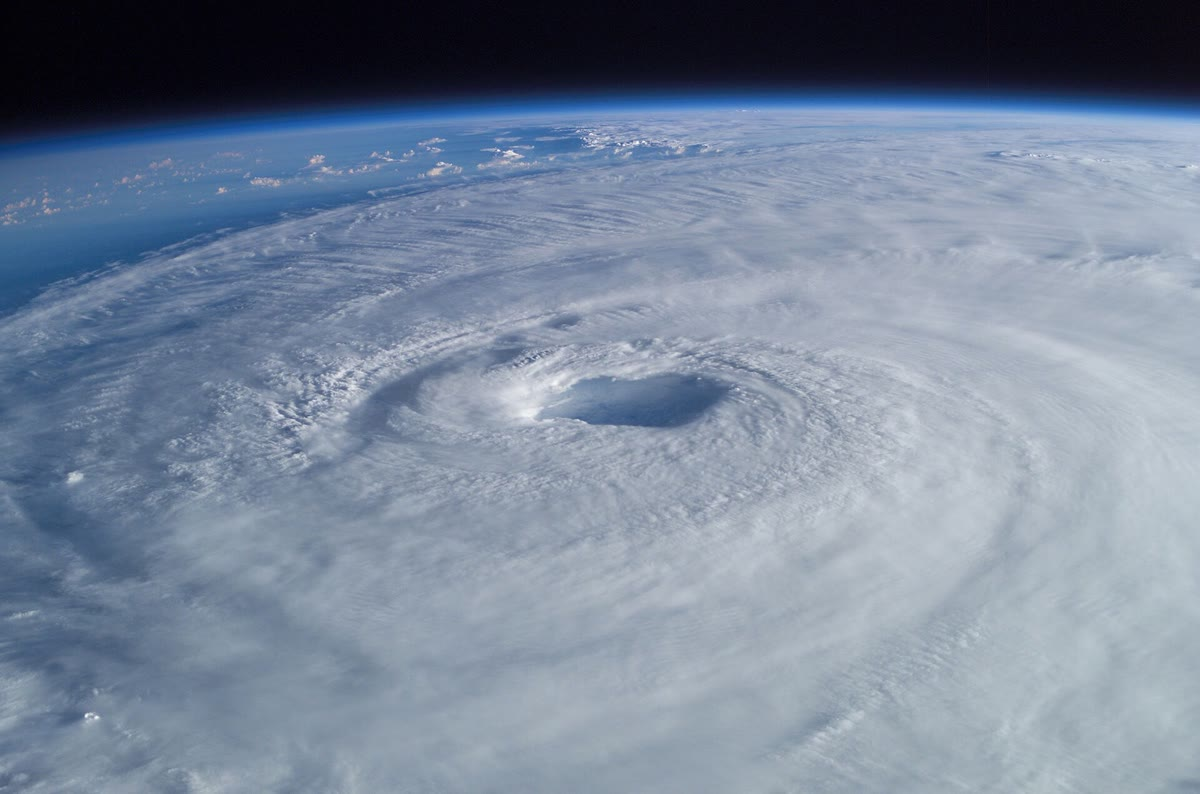
\includegraphics[width=0.78\linewidth]{images/book2/g10-nasa-hurricane-isabel.jpg}

{\small L'ouragan Isabel, le 15~septembre 2003, photographié par un
astronaute depuis la Station spatiale internationale~: l'\omterm{def:g10:storms-and-cyclones:tropical-cyclone}{œil}, le \omterm{def:g10:storms-and-cyclones:tropical-cyclone}{mur de
l'œil} et la spirale de nuages qui les entoure. Image~: Mike Trenchard, Earth
Sciences and Image Analysis Laboratory, NASA Johnson Space Center (domaine
public).}
\end{omfigure}

Près de la surface de la mer, l'air humide afflue vers la basse pression du
centre. La rotation de la Terre dévie l'air en mouvement vers la droite dans
l'hémisphère Nord~: au lieu d'aller droit au centre, l'air tourne autour,
dans le sens inverse des aiguilles d'une montre vu d'en haut (dans le sens
des aiguilles d'une montre dans l'hémisphère Sud). Près du centre, il monte
dans le \omterm{def:g10:storms-and-cyclones:tropical-cyclone}{mur de l'œil}, se condense et s'écoule au sommet de la tempête. Dans
l'\omterm{def:g10:storms-and-cyclones:tropical-cyclone}{œil}, un peu d'air descend, se réchauffe et s'assèche~: le ciel se dégage.

\begin{omfigure}
\begin{tikzpicture}[font=\footnotesize, >={Stealth[length=2mm]}]
  \fill[omDef!25] (-6,-0.4) rectangle (6,0);
  \node[anchor=north, omDef!80!black] at (0,-0.05) {mer chaude};
  % rain bands
  \foreach \x/\h in {-5.0/1.6, -3.9/2.2, 3.9/2.2, 5.0/1.6}
    \fill[black!10, draw=black!45] (\x-0.35,0.4) -- (\x-0.3,\h) .. controls (\x-0.15,\h+0.35) and (\x+0.15,\h+0.35) .. (\x+0.3,\h) -- (\x+0.35,0.4) -- cycle;
  % eyewall towers and outflow canopy
  \fill[black!14, draw=black!50] (-2.4,0.4) -- (-2.5,4.0) -- (-5.8,4.3) -- (-5.6,4.7) -- (-1.0,4.9) -- (-0.75,4.0) -- (-0.8,0.4) -- cycle;
  \fill[black!14, draw=black!50] (2.4,0.4) -- (2.5,4.0) -- (5.8,4.3) -- (5.6,4.7) -- (1.0,4.9) -- (0.75,4.0) -- (0.8,0.4) -- cycle;
  % inflow, rise, outflow, eye subsidence
  \draw[->, thick, omThm!80!black] (-5.8,0.2) -- (-1.3,0.2) -- (-1.3,4.3) -- (-4.2,4.45);
  \draw[->, thick, omThm!80!black] (5.8,0.2) -- (1.3,0.2) -- (1.3,4.3) -- (4.2,4.45);
  \draw[->, thick, omDef!80!black] (0,4.3) -- (0,1.0);
  \node[anchor=south, align=center] at (0,5.0) {œil~: air sec\\descendant};
  \node[anchor=south east, align=right] at (-2.6,4.95) {mur de l'œil};
  \node[anchor=west, align=left] at (-5.95,2.9) {bandes\\de pluie};
  \node[anchor=north, align=center] at (-3.6,0.15) {afflux humide};
  \node[anchor=south east, align=right] at (5.8,4.95) {divergence en altitude};
  % plan view
  \begin{scope}[shift={(8.4,2.3)}]
    \draw[black!40] (0,0) circle (1.7);
    \foreach \a in {0,90,180,270}
      \draw[->, thick, omThm!80!black, domain=0:200, samples=30, variable=\t]
        plot ({(1.6-0.0045*\t)*cos(\a+\t)}, {(1.6-0.0045*\t)*sin(\a+\t)});
    \fill[white, draw=black!50] (0,0) circle (0.22);
    \node[anchor=north, align=center] at (0,-1.8) {vu d'en haut\\(hémisphère Nord)};
  \end{scope}
\end{tikzpicture}

{\small Un \omterm{def:g10:storms-and-cyclones:tropical-cyclone}{cyclone tropical} en coupe (schéma, hauteurs très exagérées)~:
l'air humide afflue au-dessus de la mer chaude, monte dans le \omterm{def:g10:storms-and-cyclones:tropical-cyclone}{mur de l'œil}
et les bandes de pluie, et s'écoule au sommet~; un peu d'air descend dans
l'\omterm{def:g10:storms-and-cyclones:tropical-cyclone}{œil}. À droite~: vu d'en haut dans l'hémisphère Nord, l'air qui afflue
tourne autour du centre dans le sens inverse des aiguilles d'une montre.}
\end{omfigure}

Les \omterm{def:g10:storms-and-cyclones:tropical-cyclone}{cyclones tropicaux} ont besoin d'un océan chaud~: une eau d'au moins
\qty{27}{\degreeCelsius} environ en surface, chaude jusqu'à une profondeur
de quelque \qty{46}{m}. Ils ne se forment pas sur l'équateur même, où la
rotation de la Terre n'imprime aucune déviation à l'air qui afflue~: une
tempête doit être à au moins \qty{480}{km} environ de l'équateur pour que
la rotation s'amorce.
% ledger: aoml:formation

\begin{omfigure}
\begin{tikzpicture}
\begin{axis}[ommap, width=\linewidth, xtick={-180,-120,...,180}, ytick={-60,-30,0,30,60},
  ymin=-70, ymax=70, unbounded coords=jump]
\addplot[fill=omLithAlluv, draw=black!45, line width=0.2pt] table {figdata/out/shared-geo-land.dat};
\addplot[omThm!70, line width=0.25pt] table {figdata/out/grade-10-cyclones-tracks.dat};
\addplot[only marks, mark=*, mark size=0.45pt, omDef!90!black] table {figdata/out/grade-10-cyclones-genesis.dat};
\addplot[black!45, dashed, domain=-180:180] {0};
\end{axis}
\end{tikzpicture}

{\small \omterm{def:g10:storms-and-cyclones:tropical-cyclone}{Cyclones tropicaux}~: les trajectoires de toutes les tempêtes des
saisons 2015--2024 (en rouge), et le lieu où chaque tempête des saisons
1980--2024 a atteint pour la première fois l'intensité de tempête tropicale
(points bleus). Données~: IBTrACS v04r01, NOAA National Centers for
Environmental Information.}
\end{omfigure}
% ledger: data:b2-ibtracs (all statistics computed in figdata/grade-10/cyclones.py)

La carte montre la règle à l'œuvre. Sur les 3\,888 tempêtes de 1980--2024,
24 seulement ont atteint l'intensité de tempête tropicale à moins de
\qty{5}{\degree} de l'équateur. La plupart se forment entre \qty{10}{\degree}
et \qty{30}{\degree} de latitude, puis dérivent vers l'ouest avec les
alizés et s'incurvent vers les pôles, où la mer froide les affaiblit.
L'Atlantique Sud, plus frais et moins favorable, n'en a vu que trois en
45~ans. Il se forme environ 87 \omterm{def:g10:storms-and-cyclones:tropical-cyclone}{cyclones tropicaux} par an en moyenne, sept
sur dix dans l'hémisphère Nord, et un peu plus de la moitié atteignent
l'intensité d'ouragan.

\begin{proposition}[La source d'énergie d'un cyclone tropical]\label{prop:g10:storms-and-cyclones:energy}
Un \omterm{def:g10:storms-and-cyclones:tropical-cyclone}{cyclone tropical} tire son énergie de la mer chaude~: la \omterm{def:g10:earth-energy-budget:latent-heat}{chaleur latente}
prise par l'évaporation à la surface de la mer est libérée dans le \omterm{def:g10:storms-and-cyclones:tropical-cyclone}{mur de
l'œil} et les bandes de pluie quand la vapeur se condense. Un ouragan moyen
libère ainsi environ \qty{6e14}{W}~; une petite fraction seulement, environ
\qty{1.5e12}{W}, devient de l'énergie cinétique de ses vents.
\end{proposition}
% ledger: aoml:energy

\begin{proof}[Justification]
Un ouragan moyen déverse \qty{1.5}{cm} de pluie par jour sur un disque de
rayon \qty{665}{km}, d'aire $\pi \times (665\,000)^2 \approx
\qty{1.39e12}{m^2}$~: \qty{2.1e10}{m^3}, soit \qty{2.1e13}{kg}, d'eau par
jour. Chaque kilogramme qui se condense libère environ \qty{2.5}{MJ}~:
$2.1\times10^{13}
\times 2.5\times10^6 \approx \qty{5.2e19}{J}$ par jour, c'est-à-dire
$5.2\times10^{19}/86\,400 \approx \qty{6.0e14}{W}$. La puissance des vents
est une estimation tirée de champs de vent mesurés, citée d'après la même
source.
\end{proof}

La tempête fonctionne comme un moteur~: de la chaleur prise à la surface
chaude de la mer, cédée très haut dans l'air froid d'altitude, une partie de
la différence étant transformée en mouvement du vent. C'est pourquoi un
\omterm{def:g10:storms-and-cyclones:tropical-cyclone}{cyclone tropical} s'affaiblit vite quand il passe sur la terre ferme ou sur
une eau froide~: il perd son apport d'eau qui s'évapore.

\section{Intensité, vents et ondes de tempête}

\begin{definition}[Échelle de Saffir--Simpson]\label{def:g10:storms-and-cyclones:scale}
L'\emph{échelle de Saffir--Simpson}\index{echelle de Saffir--Simpson@échelle de Saffir--Simpson}
classe les ouragans en cinq catégories selon leur vent soutenu maximal~;
les catégories 3 à 5 sont les ouragans \emph{majeurs}.
\end{definition}

\begin{center}
\small
\begin{tabular}{cccc}
\hline
catégorie & nœuds & \unit{m/s} & \unit{km/h} \\
\hline
1 & 64--82 & 33--42 & 119--153 \\
2 & 83--95 & 43--49 & 154--177 \\
3 & 96--112 & 49--58 & 178--208 \\
4 & 113--136 & 58--70 & 209--251 \\
5 & 137 ou plus & 70 ou plus & 252 ou plus \\
\hline
\end{tabular}
\end{center}
% ledger: nhc:sshws (m/s converted with 1 knot = 1852/3600 m/s)

Plus la basse pression du centre est profonde, plus les vents qui soufflent
autour sont forts~: c'est la différence de pression entre le centre et les
alentours qui pousse l'air vers l'intérieur.

\begin{omfigure}
\begin{tikzpicture}
\begin{axis}[omrecord, width=0.86\linewidth, height=6.2cm, xmin=15, xmax=100,
  ymin=860, ymax=1015, xlabel={vent soutenu maximal (\unit{m/s})},
  ylabel={pression centrale minimale (\unit{hPa})},
  tick label style={font=\small}, label style={font=\small}]
\foreach \w in {32.92, 42.70, 49.39, 58.13, 70.48}
  \edef\temp{\noexpand\draw[black!55, densely dashed] (axis cs:\w,860) -- (axis cs:\w,1015);}\temp
\addplot[only marks, mark=*, mark size=0.6pt, omDef!80!black, opacity=0.6] table[x=wind_ms, y=pmin_hpa] {figdata/out/grade-10-cyclones-scatter.dat};
\addplot[omThm!85!black, thick] table[x=wind_ms, y=pmin_hpa] {figdata/out/grade-10-cyclones-fit.dat};
\node[font=\scriptsize, black!60] at (axis cs:37.8,1008) {1};
\node[font=\scriptsize, black!60] at (axis cs:46.0,1008) {2};
\node[font=\scriptsize, black!60] at (axis cs:53.8,1008) {3};
\node[font=\scriptsize, black!60] at (axis cs:64.3,1008) {4};
\node[font=\scriptsize, black!60] at (axis cs:76,1008) {5};
\end{axis}
\end{tikzpicture}

{\small Chaque point est un \omterm{def:g10:storms-and-cyclones:tropical-cyclone}{cyclone tropical} des saisons 2000--2024~: son
vent soutenu le plus fort et sa pression centrale la plus basse. La droite
est le meilleur ajustement linéaire~: environ \qty{1.6}{hPa} de moins par
mètre par seconde supplémentaire. Tirets gris~: les limites des catégories
de Saffir--Simpson (numérotées en haut). Données~: IBTrACS v04r01, NOAA
NCEI.}
\end{omfigure}
% ledger: data:b2-ibtracs, nhc:sshws (fit computed in figdata/grade-10/cyclones.py)

Le record des tempêtes 1980--2024 de l'archive revient à l'ouragan
Patricia, au large de la côte pacifique du Mexique en octobre 2015~: des
vents soutenus de 185~nœuds, environ \qty{95}{m/s}, et une pression centrale
de \qty{872}{hPa}.
% ledger: data:b2-ibtracs

\begin{definition}[Onde de tempête]\label{def:g10:storms-and-cyclones:storm-surge}
Une \emph{onde de tempête}\index{onde de tempete@onde de tempête}, ou
surcote, est l'élévation de la mer au-dessus de son niveau normal, marée
exclue, causée par une tempête~: le vent accumule l'eau contre la côte, et
la basse pression laisse la mer se bomber sous la tempête.
\end{definition}

\begin{proposition}[Le bombement de pression]\label{prop:g10:storms-and-cyclones:bulge}
Sous une tempête dont la pression centrale est inférieure de $\Delta p$
hectopascals à celle des alentours, la mer monte d'environ $\Delta p$
centimètres.
\end{proposition}

\begin{proof}
Loin sous la surface, la pression doit être la même sous la tempête et en
dehors, sinon l'eau s'écoulerait. L'air au-dessus de la tempête pèse
$\Delta p$ de moins~; une colonne d'eau de mer de hauteur $h$ compense ce
déficit si
$\rho g h = \Delta p$. Pour $\Delta p = \qty{1}{hPa} = \qty{100}{Pa}$, avec
$\rho = \qty{1025}{kg/m^3}$ et $g = \qty{9.81}{m/s^2}$~: $h = 100/(1025
\times 9.81) \approx \qty{0.0099}{m}$, environ \qty{1}{cm}.
\end{proof}
% ledger: noaa:seawater-1025, nasa:aquarius-density, const:gn

Le bombement est la plus petite part de la plupart des \omterm{def:g10:storms-and-cyclones:storm-surge}{ondes de tempête}~:
sous une pression centrale de \qty{920}{hPa}, inférieure de \qty{90}{hPa}
à celle des alentours, il atteint environ \qty{0.9}{m}. Le vent fait le
reste, en poussant l'eau vers le rivage, surtout au-dessus d'un fond marin
large et peu profond. Si elle arrive avec une marée haute, une \omterm{def:g10:storms-and-cyclones:storm-surge}{onde de
tempête} de plusieurs mètres peut inonder des côtes basses loin à
l'intérieur des terres.

\begin{omfigure}
\begin{tikzpicture}[font=\footnotesize, >={Stealth[length=2mm]}]
  \def\surf{(0,0) .. controls (1.5,0) and (2.2,0.5) .. (3.0,0.5) .. controls (3.8,0.5) and (4.6,0.4) .. (5.6,0.5) .. controls (7.2,0.65) and (8.8,1.0) .. (10.25,1.3)}
  \fill[omDef!20] (0,-1.6) -- \surf -- (8.8,-1.6) -- cycle;
  \draw[thick, omDef!80!black] \surf;
  \draw[black!50, dashed] (0,0) -- (9.6,0);
  \node[anchor=north west, black!60] at (0.1,-0.05) {niveau normal de la mer};
  \fill[omExo!30, draw=black!60] (8.8,-1.6) -- (10.4,1.6) -- (12.4,1.7) -- (12.4,-1.6) -- cycle;
  \foreach \x in {10.9,11.7} \draw[fill=white, draw=black!60] (\x,1.63) rectangle (\x+0.45,2.03) (\x-0.05,2.03) -- (\x+0.225,2.28) -- (\x+0.5,2.03);
  \draw[<->, omThm!80!black] (3.0,0) -- (3.0,0.5);
  \node[anchor=south east, omThm!80!black, align=right] at (2.8,0.6) {bombement sous\\la basse pression};
  \draw[<->, omThm!80!black] (9.4,0) -- (9.4,1.12);
  \node[anchor=south, omThm!80!black, align=center] at (8.9,1.75) {surélévation due\\au vent contre la côte};
  \foreach \y in {2.9,3.4} \draw[->, thick, black!60] (4.0,\y) -- (6.4,\y);
  \node[anchor=south] at (5.2,3.45) {vent de mer};
  \node[anchor=south, align=center] at (3.0,1.9) {centre de\\la tempête};
  \draw[black!40] (3.0,1.9) -- (3.0,0.65);
\end{tikzpicture}

{\small Une \omterm{def:g10:storms-and-cyclones:storm-surge}{onde de tempête} (schéma, hauteurs très exagérées)~: la mer monte
d'environ \qty{1}{cm} par hectopascal de basse pression sous la tempête, et
le vent de mer accumule l'eau contre la côte.}
\end{omfigure}

\begin{omfigure}
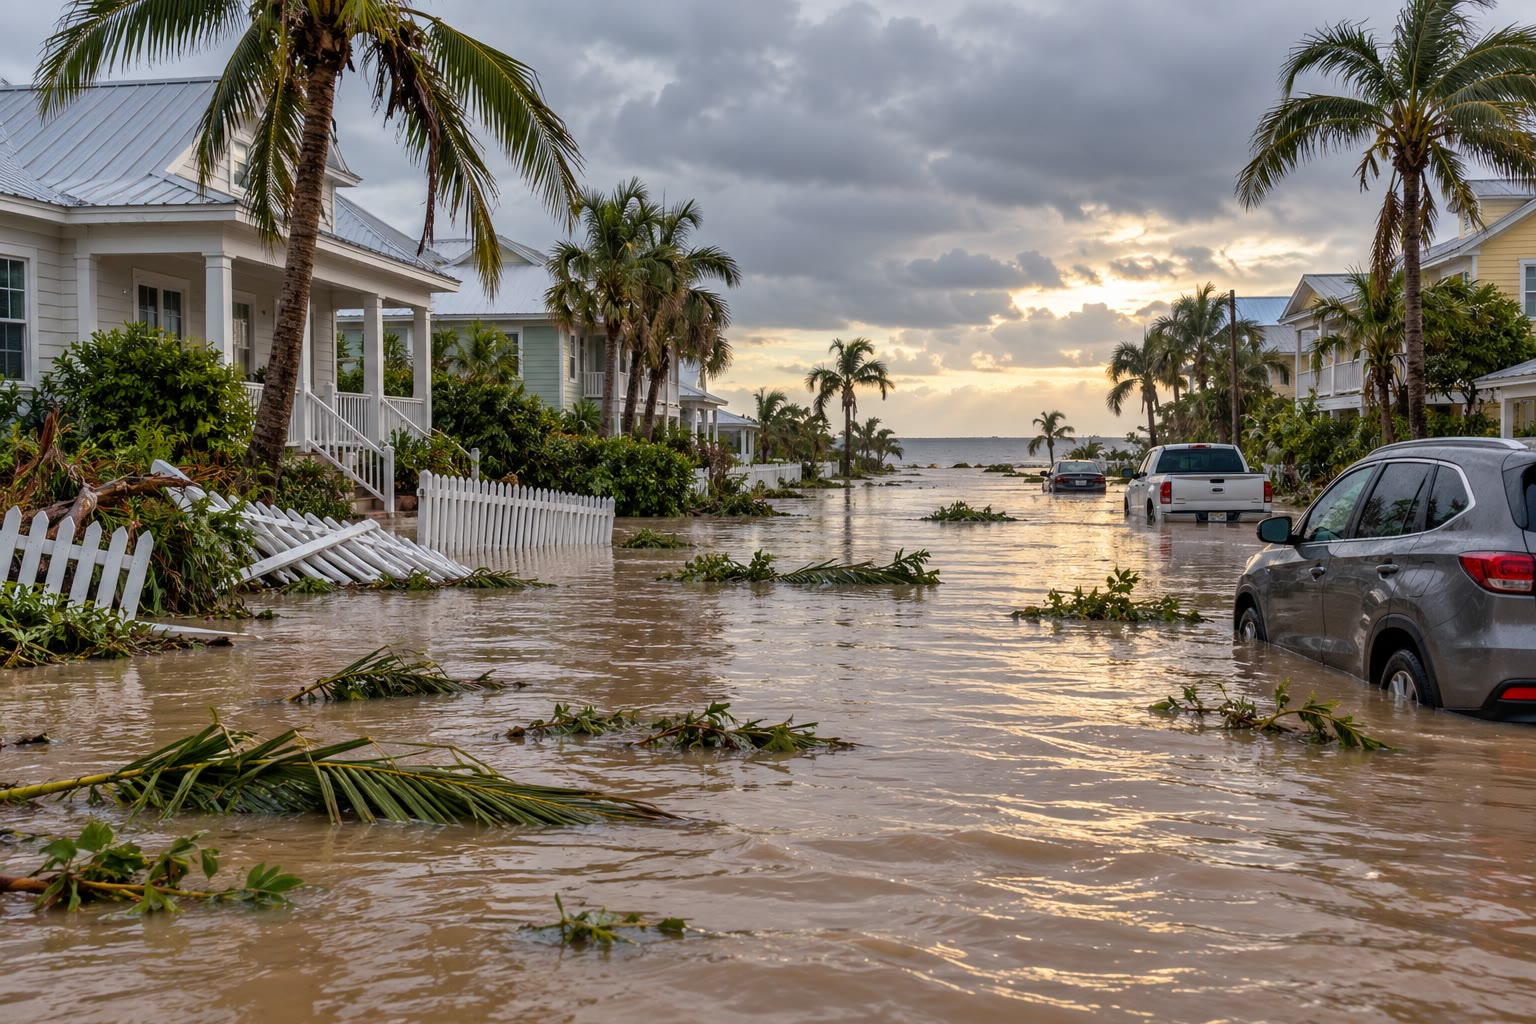
\includegraphics[width=0.7\linewidth]{images/book2/ai/g10-flooded-street.jpg}

{\small Une rue côtière au lendemain d'une \omterm{def:g10:storms-and-cyclones:storm-surge}{onde de tempête}~: eau de mer,
palmiers brisés et clôtures arrachées.}
\end{omfigure}

\section{Exercices}

\begin{exercise}[$\star$]\label{exo:g10:storms-and-cyclones:1}
Définir un \omterm{def:g10:storms-and-cyclones:thunderstorm}{orage} et un \omterm{def:g10:storms-and-cyclones:lightning}{éclair}. Qu'est-ce qui produit le bruit du tonnerre~?
\end{exercise}

\begin{exercise}[$\star$]\label{exo:g10:storms-and-cyclones:2}
Définir un \omterm{def:g10:storms-and-cyclones:tropical-cyclone}{cyclone tropical}, son \omterm{def:g10:storms-and-cyclones:tropical-cyclone}{œil} et son \omterm{def:g10:storms-and-cyclones:tropical-cyclone}{mur de l'œil}. Où ses vents
sont-ils les plus forts~?
\end{exercise}

\begin{exercise}[$\star$]\label{exo:g10:storms-and-cyclones:3}
Dans quelle catégorie de Saffir--Simpson se range un ouragan aux vents
soutenus de \num{70}~nœuds~? De \num{120}~nœuds~? De \num{140}~nœuds~?
Lesquels sont des ouragans majeurs~?
\end{exercise}

\begin{exercise}[$\star$]\label{exo:g10:storms-and-cyclones:4}
On compte \num{9} secondes entre un \omterm{def:g10:storms-and-cyclones:lightning}{éclair} et son tonnerre, puis \num{15}
secondes pour l'\omterm{def:g10:storms-and-cyclones:lightning}{éclair} suivant. À quelle distance était chacun, et l'\omterm{def:g10:storms-and-cyclones:thunderstorm}{orage}
se rapproche-t-il~?
\end{exercise}

\begin{exercise}[$\star$]\label{exo:g10:storms-and-cyclones:5}
Expliquer pourquoi un arbre isolé dans un champ est un abri dangereux
pendant un \omterm{def:g10:storms-and-cyclones:thunderstorm}{orage}, et où il faut aller à la place.
\end{exercise}

\begin{exercise}[$\star\star$]\label{exo:g10:storms-and-cyclones:6}
Un nœud vaut \qty{1852}{m} par heure. Convertir \num{64}~nœuds et
\num{137}~nœuds en \unit{m/s} et en \unit{km/h}.
\end{exercise}

\begin{exercise}[$\star\star$]\label{exo:g10:storms-and-cyclones:7}
Il se produit 44 \omterm{def:g10:storms-and-cyclones:lightning}{éclairs} par seconde sur la Terre. Combien cela fait-il en
un jour, et en un an~?
\end{exercise}

\begin{exercise}[$\star\star$]\label{exo:g10:storms-and-cyclones:8}
Un ouragan a une pression centrale de \qty{935}{hPa} dans un environnement
à \qty{1010}{hPa}. Quelle est la hauteur du bombement de la mer sous lui~?
\end{exercise}

\begin{exercise}[$\star\star$]\label{exo:g10:storms-and-cyclones:9}
À l'aide de la carte des trajectoires, décrire où se forment les \omterm{def:g10:storms-and-cyclones:tropical-cyclone}{cyclones
tropicaux} et où ils vont ensuite. Pourquoi sont-ils absents de l'équateur
même~?
\end{exercise}

\begin{exercise}[$\star\star$]\label{exo:g10:storms-and-cyclones:10}
La droite du graphique pression--vent est $p \approx 1031 - 1.56\,v$
($p$ en \unit{hPa}, $v$ en \unit{m/s}). Quelle pression centrale donne-t-elle
pour la limite inférieure de la catégorie 5, \qty{70}{m/s}~? Pour une
tempête de \qty{40}{m/s}~?
\end{exercise}

\begin{exercise}[$\star\star$]\label{exo:g10:storms-and-cyclones:11}
Expliquer pourquoi un \omterm{def:g10:storms-and-cyclones:tropical-cyclone}{cyclone tropical} s'affaiblit vite quand il passe sur
la terre ferme, et pourquoi il s'affaiblit au-dessus d'une eau froide.
\end{exercise}

\begin{exercise}[$\star\star\star$]\label{exo:g10:storms-and-cyclones:12}
La vitesse du son dans l'air vaut $\sqrt{1.4\,R\,T/M}$, avec $R =
\qty{8.314}{J.mol^{-1}.K^{-1}}$, $T$ en kelvins et $M =
\qty{0.02897}{kg/mol}$. La calculer à \qty{0}{\degreeCelsius} et à
\qty{30}{\degreeCelsius}. Pour un délai de \qty{9}{s}, de combien les deux
distances diffèrent-elles~? La règle «~\qty{3}{s} par kilomètre~»
suffit-elle~?
\end{exercise}

\begin{exercise}[$\star\star\star$]\label{exo:g10:storms-and-cyclones:13}
Une \omterm{def:g10:storms-and-cyclones:storm-surge}{onde de tempête} de \qty{4.0}{m} est mesurée sur une côte au moment où
un ouragan de pression centrale \qty{940}{hPa} (alentours \qty{1010}{hPa})
touche terre. Quelle part de l'onde est due au bombement de pression, et
quelle part au vent~? Si elle arrive à marée haute, \qty{1.5}{m} au-dessus
du niveau moyen de la mer, jusqu'à quelle hauteur au-dessus du niveau moyen
l'eau monte-t-elle~?
\end{exercise}

\begin{exercise}[$\star\star\star$]\label{exo:g10:storms-and-cyclones:14}
Une \omterm{def:g10:storms-and-cyclones:tornado}{tornade} tourne avec des vents de \qty{90}{m/s} à \qty{100}{m} de son
axe~; un ouragan, avec des vents de \qty{60}{m/s} dans un \omterm{def:g10:storms-and-cyclones:tropical-cyclone}{mur de l'œil} situé
à \qty{30}{km} du centre. Combien de temps l'air met-il à faire un tour dans
chaque cas~? Comparer.
\end{exercise}

\begin{exercise}[$\star\star\star$]\label{exo:g10:storms-and-cyclones:15}
Sur les 3\,888 \omterm{def:g10:storms-and-cyclones:tropical-cyclone}{cyclones tropicaux} de 1980--2024, 24 ont atteint
l'intensité de tempête tropicale à moins de \qty{5}{\degree} de l'équateur,
414 à moins de \qty{10}{\degree}, et 121 au-delà de \qty{30}{\degree}.
Calculer les trois pourcentages. La bande située à moins de
\qty{5}{\degree} de l'équateur couvre environ \qty{9}{\percent} de la
surface de la Terre~: à quoi s'attendrait-on si la latitude ne comptait
pas, et que peut-on en conclure~?
\end{exercise}

\section{Problème~: le moteur thermique d'un ouragan}

\begin{problem}[{Problème du week-end --- de la pluie d'une journée à la
puissance du vent}]
\label{pb:g10:storms-and-cyclones:1}
% ledger: aoml:energy, nist:water-latent, earth:Rmean, ipcc:budget-toa (all results computed in figdata/grade-10/cyclones.py or from the rounded data below)
Un ouragan moyen déverse \qty{1.5}{cm} de pluie par jour sur un disque de
rayon \qty{665}{km}. On prendra une \omterm{def:g10:earth-energy-budget:latent-heat}{chaleur latente} de \qty{2.5}{MJ/kg},
une masse volumique de l'eau de \qty{1000}{kg/m^3}, \qty{86400}{s} dans une
journée, et la puissance des vents d'un ouragan moyen, \qty{1.5e12}{W}.

\medskip
\noindent\textbf{Partie I --- La pluie d'une journée.}
\begin{enumerate}
  \item Calculer l'aire du disque.
  \item Calculer le volume de pluie qui y tombe en une journée.
  \item L'exprimer en kilomètres cubes.
  \item Calculer sa masse.
\end{enumerate}

\medskip
\noindent\textbf{Partie II --- La chaleur libérée.}
\begin{enumerate}[resume]
  \item Calculer la \omterm{def:g10:earth-energy-budget:latent-heat}{chaleur latente} libérée en une journée par la
        condensation de cette eau.
  \item La convertir en puissance.
  \item La Terre entière absorbe environ \qty{1.22e17}{W} de lumière
        solaire (\cref{ch:g10:earth-energy-budget}). Quelle fraction en
        libère un seul ouragan~?
  \item La lumière solaire absorbée vaut en moyenne \qty{240}{W/m^2}.
        Calculer la lumière solaire absorbée par l'aire de la tempête et la
        comparer à la \omterm{def:g10:earth-energy-budget:latent-heat}{chaleur latente} de la tempête.
  \item Que montre cette comparaison sur le lieu où l'énergie de la tempête
        a été recueillie~?
\end{enumerate}

\medskip
\noindent\textbf{Partie III --- D'où vient l'eau.}
\begin{enumerate}[resume]
  \item Quelle masse d'eau doit s'évaporer chaque jour pour alimenter cette
        pluie~?
  \item L'évaporation moyenne à la surface de la Terre emporte
        \qty{82}{W/m^2}. Sur quelle aire l'évaporation moyenne fournirait-elle
        la \omterm{def:g10:earth-energy-budget:latent-heat}{chaleur latente} de la tempête~? Comparer à l'aire de la tempête.
  \item À l'aide du tableau des teneurs à saturation du
        \cref{ch:g10:why-clouds-form}, comparer l'eau que contient l'air
        saturé à \qty{28}{\degreeCelsius} et à \qty{20}{\degreeCelsius}.
  \item Expliquer pourquoi les \omterm{def:g10:storms-and-cyclones:tropical-cyclone}{cyclones tropicaux} ne se forment qu'au-dessus
        des mers chaudes.
  \item Expliquer pourquoi ils s'affaiblissent sur la terre ferme.
\end{enumerate}

\medskip
\noindent\textbf{Partie IV --- Le vent.}
\begin{enumerate}[resume]
  \item Calculer l'énergie cinétique fournie aux vents en une journée.
  \item Convertir la limite inférieure de la catégorie 3, \num{96}~nœuds,
        en \unit{m/s} (\num{1}~nœud = \qty{1852}{m/h}).
  \item L'air proche de la surface de la mer a une masse volumique d'environ
        \qty{1.16}{kg/m^3}. Calculer l'énergie cinétique d'un mètre cube de
        cet air animé de cette vitesse.
  \item Comparer la \omterm{def:g10:earth-energy-budget:latent-heat}{chaleur latente} libérée en une journée à l'énergie des
        vents en une journée.
  \item Que devient le reste de la chaleur libérée~?
  \item Quelle fraction de la chaleur libérée par la condensation devient
        du vent~?
\end{enumerate}
\end{problem}
